\section{System identification}

From the modeling detailed previously, we already have a model for a nonlinear system. In order to identify it, we must defined a bump or step to be made in the input, in order to observe the systems response.

The input will be a change in the cooling water rate from 1000 lbmole/h to 950 lbmole/h. This is done at hour 5 in the simulation.

The effect this has on the system can be seen in figure \ref{fig:step_response}. For this specific step, the change in temperature was of around $\approx 1.36^\circ F$. This already confirms the intuition we've built before.

\begin{figure}[H]
    \centering
    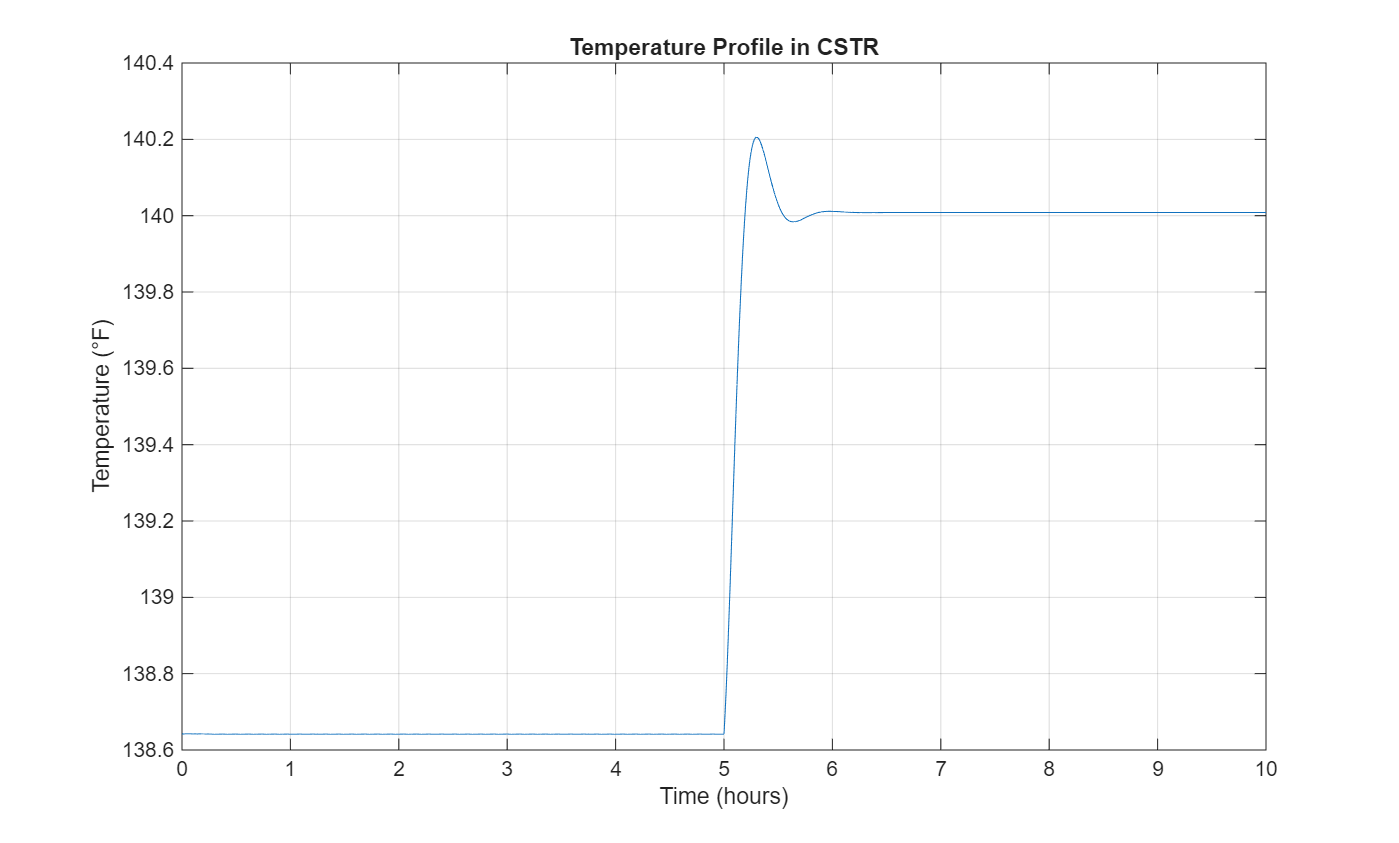
\includegraphics[width=0.8\textwidth]{../figures/Temperature profile.png}
    \caption{Reactor temperature response to a cooling water flow step from 1000 to 950 lbmol/h.}
    \label{fig:step_response}
\end{figure}

We can also check to see that the concentrations in the reactor will be affected by this change. The whole overview is not helpful, as these concentrations range a large amount (as can be seen in figure \ref{fig:step_response_concentration}), but we can zoom into the concentration profile of C, our product of interest. This can be seen in figure \ref{fig:step_response_concentration_C}. Although it is not the main focus of the exercise, we can see a change of $\approx 0.0018$ lbmole/ft$^3$ in the concentration of C.

\begin{figure}[H]
    \centering
    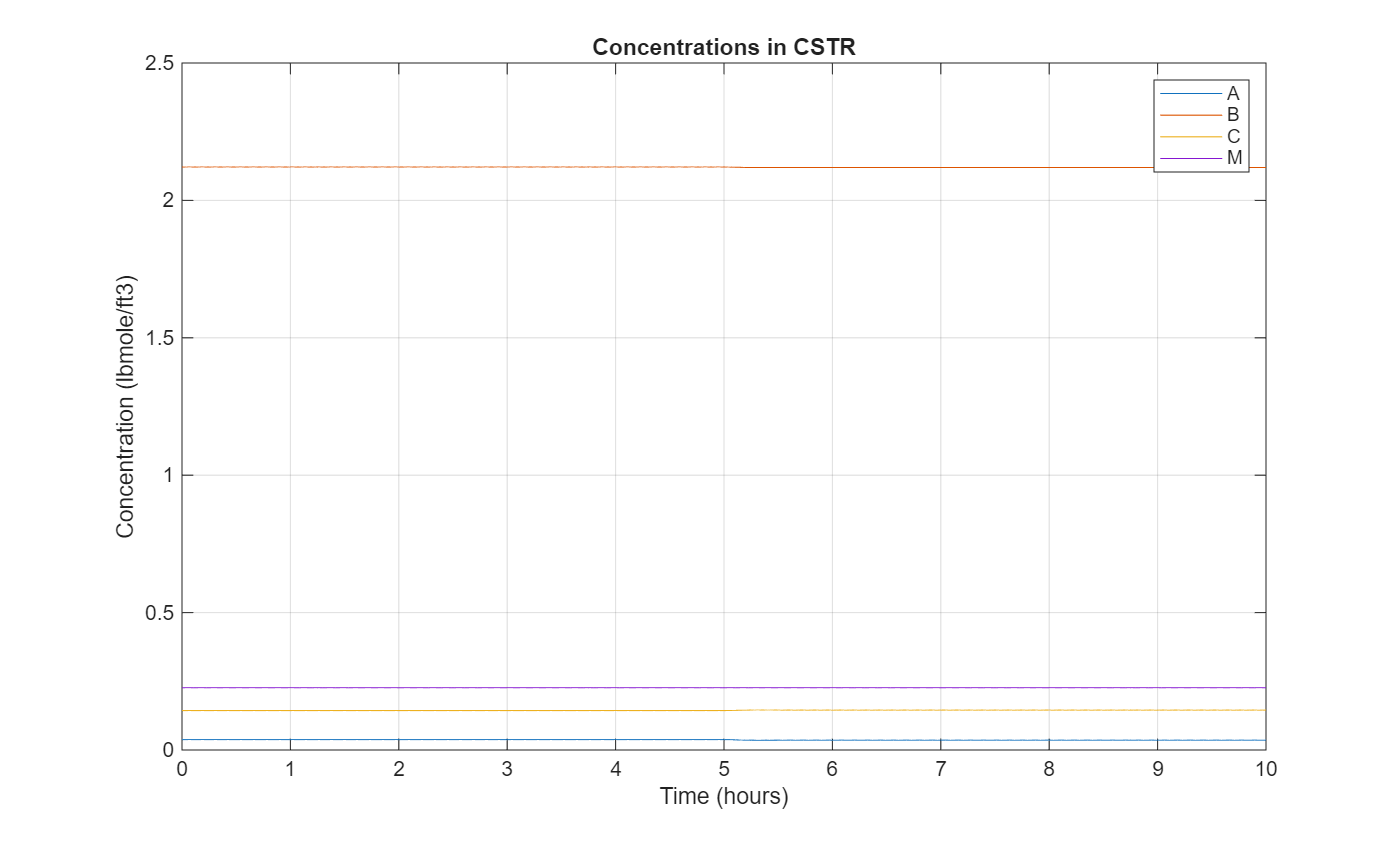
\includegraphics[width=0.8\textwidth]{../figures/Concentration profile.png}
    \caption{Concentration profiles after the cooling water flow step.}
    \label{fig:step_response_concentration}
\end{figure}

\begin{figure}[H]
    \centering
    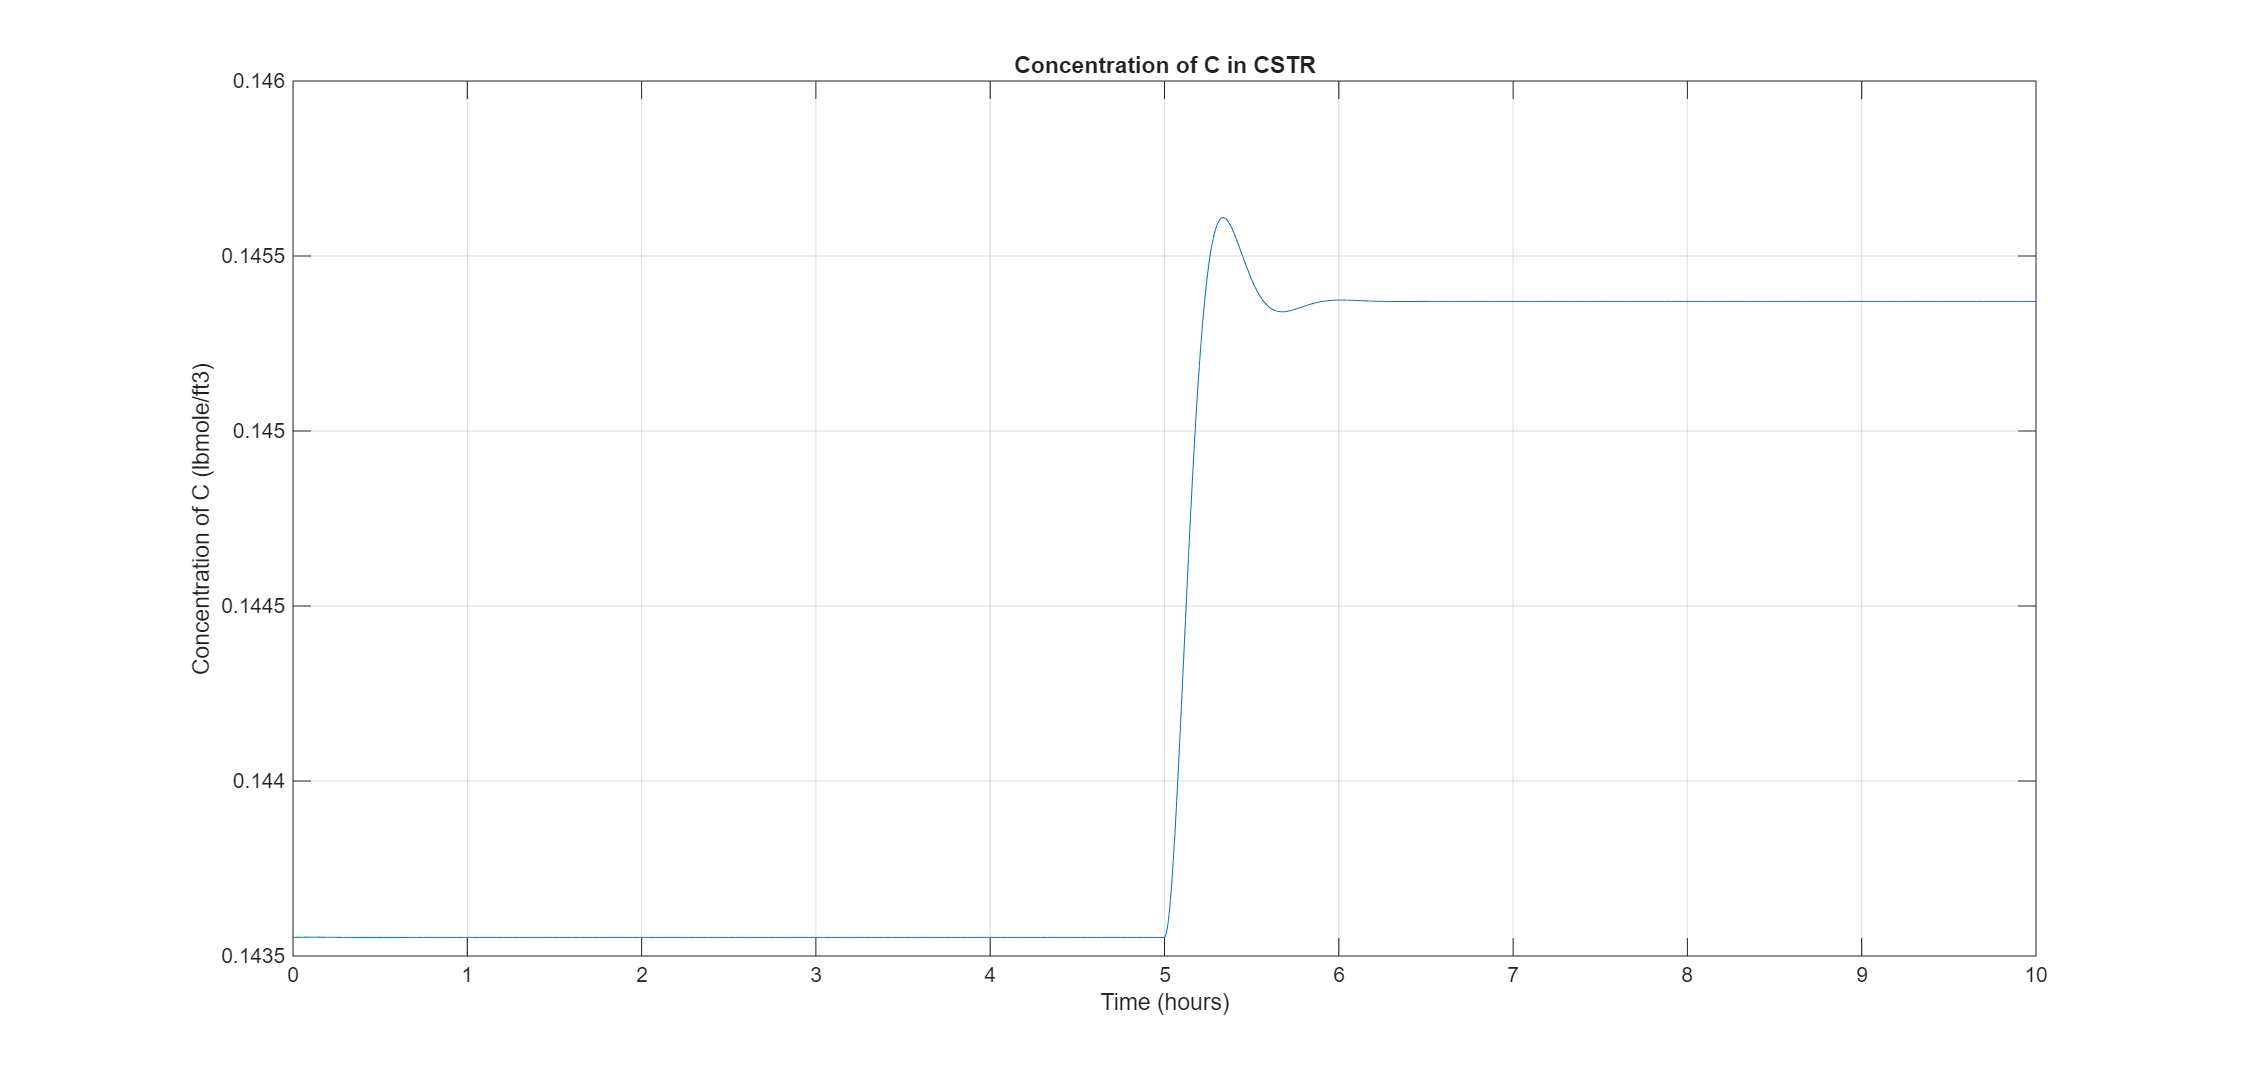
\includegraphics[width=0.8\textwidth]{../figures/Concentration profile of C.png}
    \caption{Ethylene glycol concentration response after the cooling water flow step.}
    \label{fig:step_response_concentration_C}
\end{figure}

With this data, it is possible to identify the system. The clear overshoot and settling time indicate that the system may be modeled as a second order system. Plus, a zero will be considered. 

By using MATLAB's System Identification Toolbox, we can obtain several models for the system. In this case, 3 were used: 

\begin{itemize}
    \item A first order system with just one pole.
    \item A second order system with two poles and one zero.
    \item A ARX model.
\end{itemize}

The obtained models are shown in table \ref{tab:model_comparison}. 

\begin{table}[H]
    \centering
    \caption{Comparison of identified models.}
    \label{tab:model_comparison}

    \renewcommand{\arraystretch}{2.0}
    \setlength{\tabcolsep}{12pt}

    \begin{tabular}{|C{3.6cm}|C{8.0cm}|C{2.0cm}|}
        \hline
        Model & Expression & Fit \\
        \hline

        First order no delay
        &
        $\displaystyle
        G_{1p}
        =
        \frac{-0.3036}{s+11.04}
        $
        &
        $94.35\%$
        \\
        \hline

        Second order no delay
        &
        $\displaystyle
        G_{2p1z}
        =
        \frac{-0.09353s - 3.389}{s^2 + 11.93s + 124}
        $
        &
        $99.94\%$
        \\
        \hline

        \multirow{3}{*}{ARX}
        &
        $\displaystyle
        A(z)y(t)
        =
        B(z)u(t)
        +
        e(t)
        $
        &
        \multirow{3}{*}{$100\%$}
        \\

        &
        $\displaystyle
        A(z)
        =
        1
        -
        1.878z^{-1}
        +
        0.8897z^{-2}
        $
        &
        \\

        &
        $\displaystyle
        B(z)
        =
        -0.001068z^{-1}
        +
        0.0007582z^{-2}
        $
        &
        \\
        \hline
    \end{tabular}
\end{table}

A figure that shows the comparison of the models can be seen in figure \ref{fig:1000 to 950}. 

\begin{figure}[H]
    \centering
    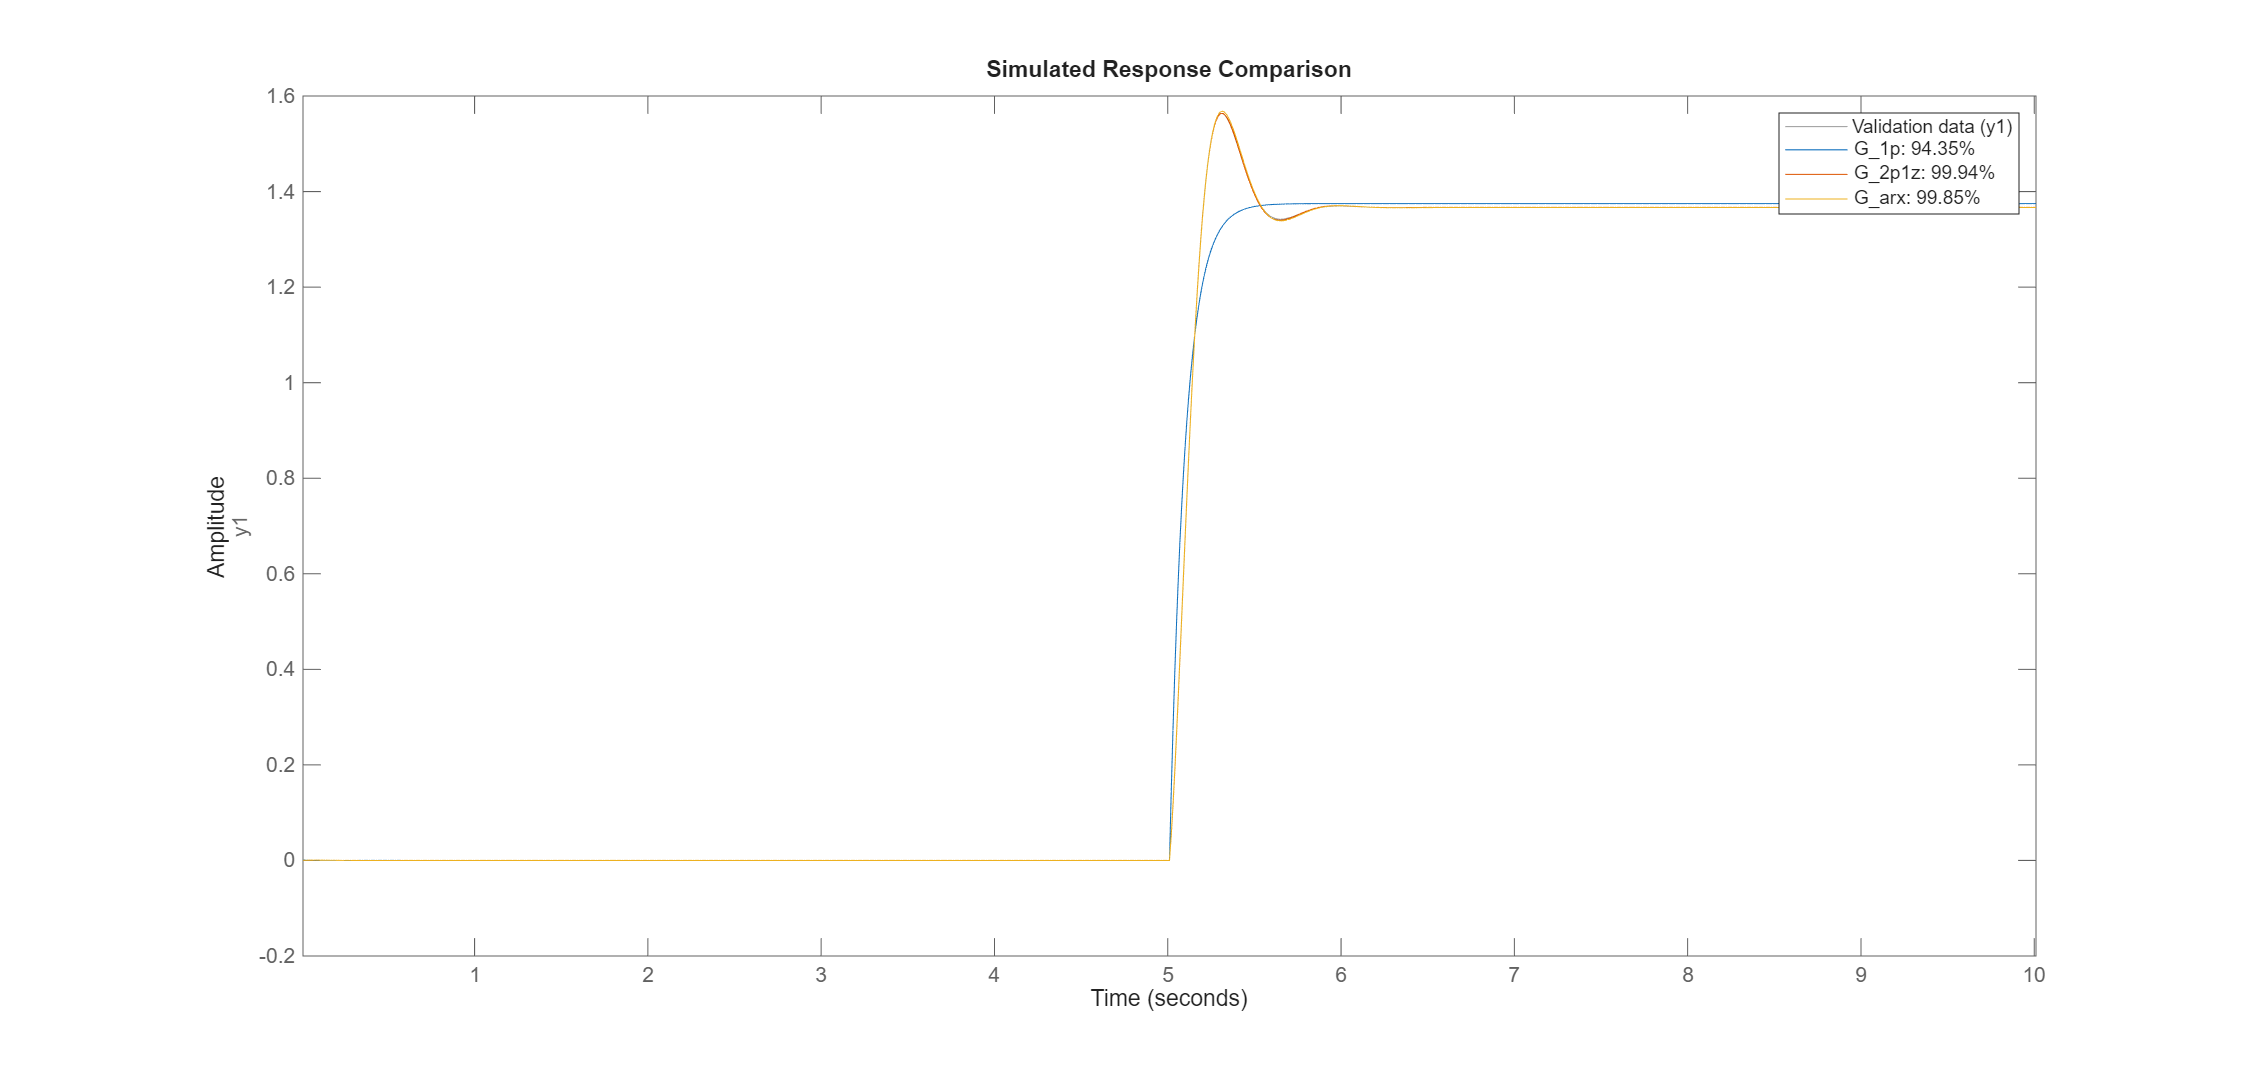
\includegraphics[width=0.8\textwidth]{../figures/1000 to 950.png}
    \caption{Model comparison for the identification dataset.}
    \label{fig:1000 to 950}
\end{figure}

\section{Validation}

From the fit, it can be inferred that the second order system with one zero is the best model for the system. The ARX model is also a good fit, but it is not as interpretable as the second order system. But nevertheless, we've just used the same data for identification and validation, so we may be incurring in some overfitting. 

For this reason, a second and third step tests were made, going from 1000 lbmole/h to 900 lbmole/h and from 1000 lbmole/h to 1050 lbmole/h. The results of these tests can be seen in figures \ref{fig:step_response_2} and \ref{fig:step_response_3}.

\begin{figure}[H]
    \centering
    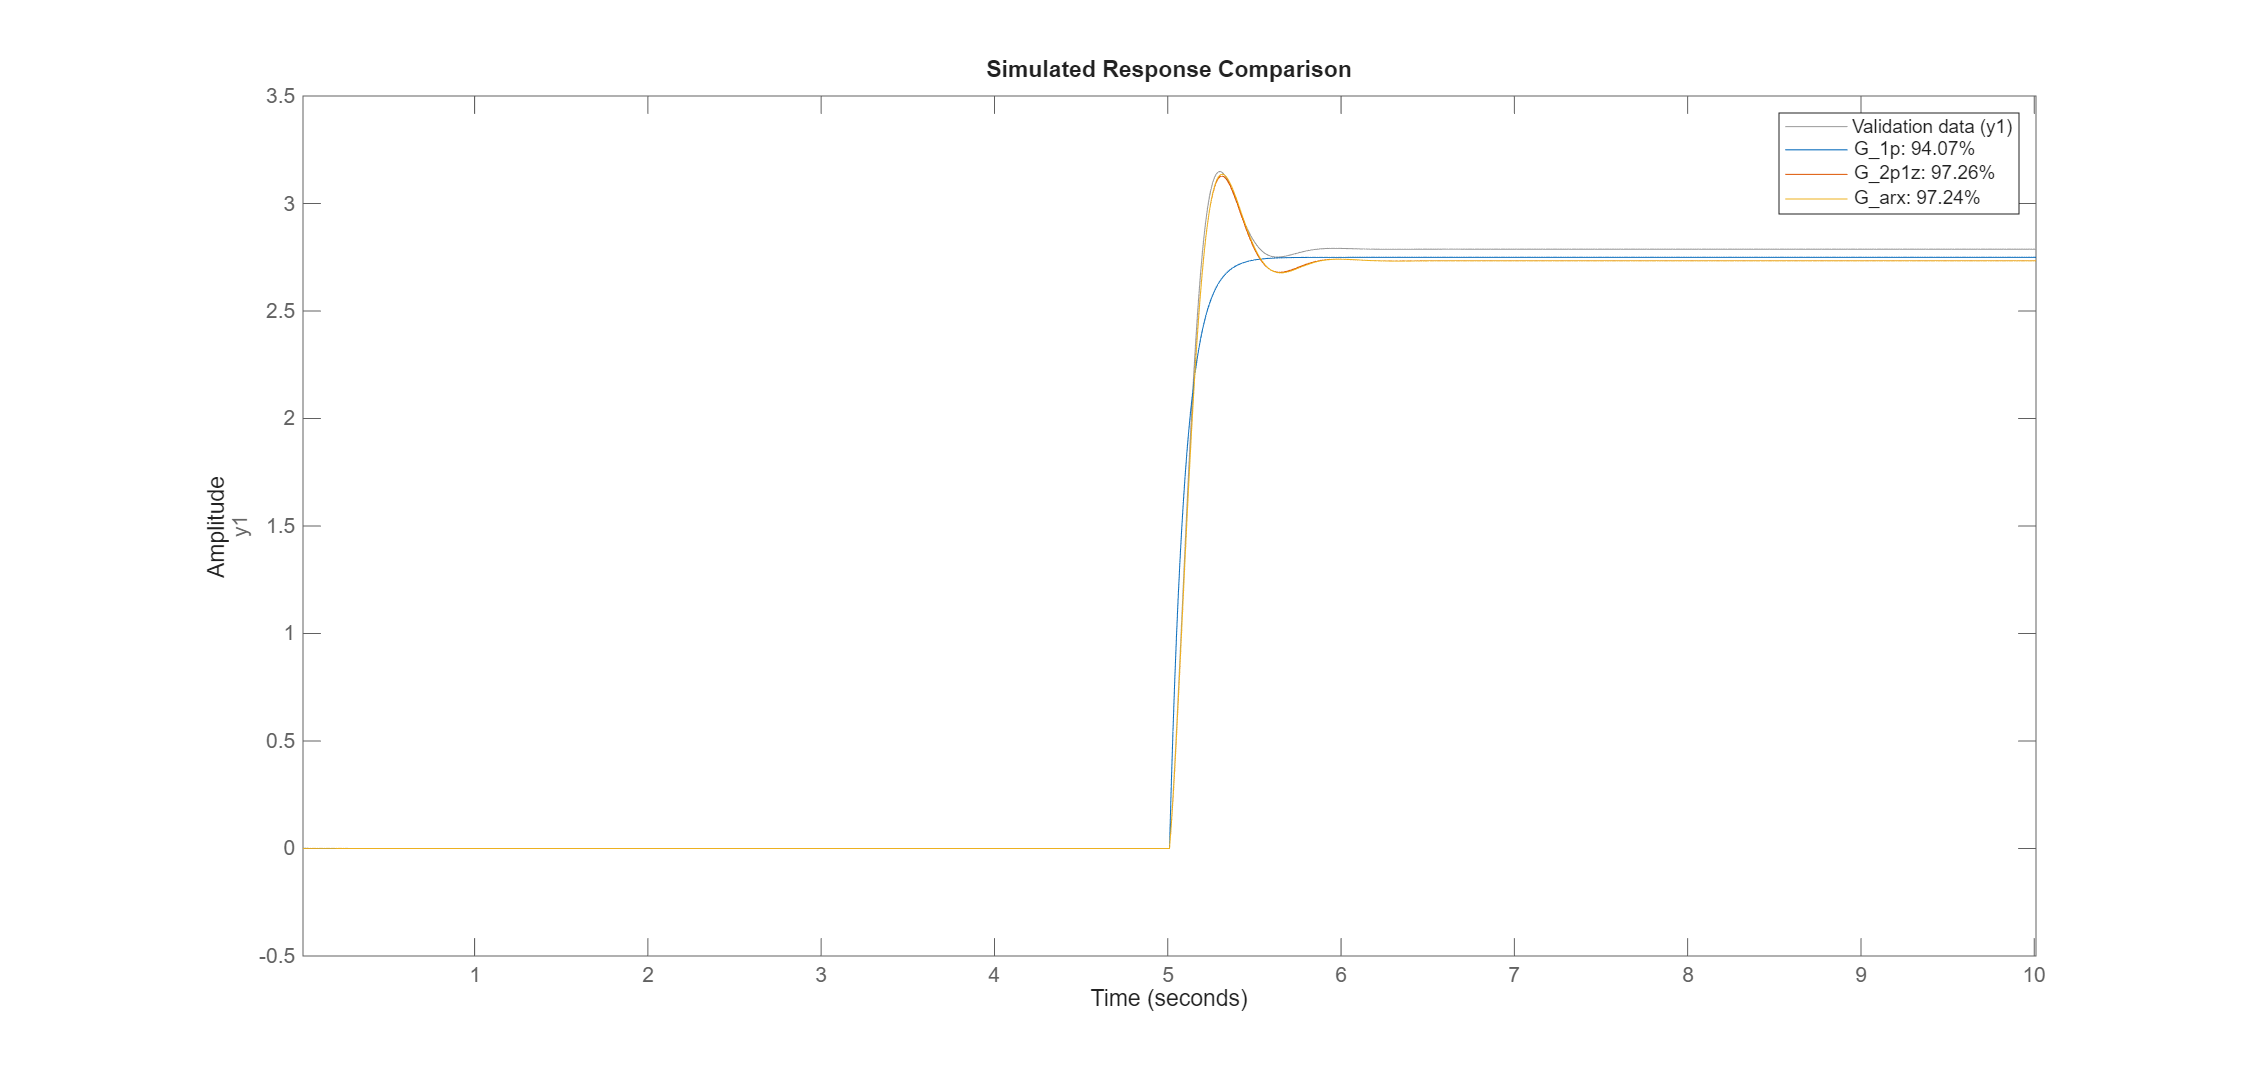
\includegraphics[width=0.8\textwidth]{../figures/1000 to 900.png}
    \caption{Validation response for cooling water flow step from 1000 to 900 lbmol/h.}
    \label{fig:step_response_2}
\end{figure}

\begin{figure}[H]
    \centering
    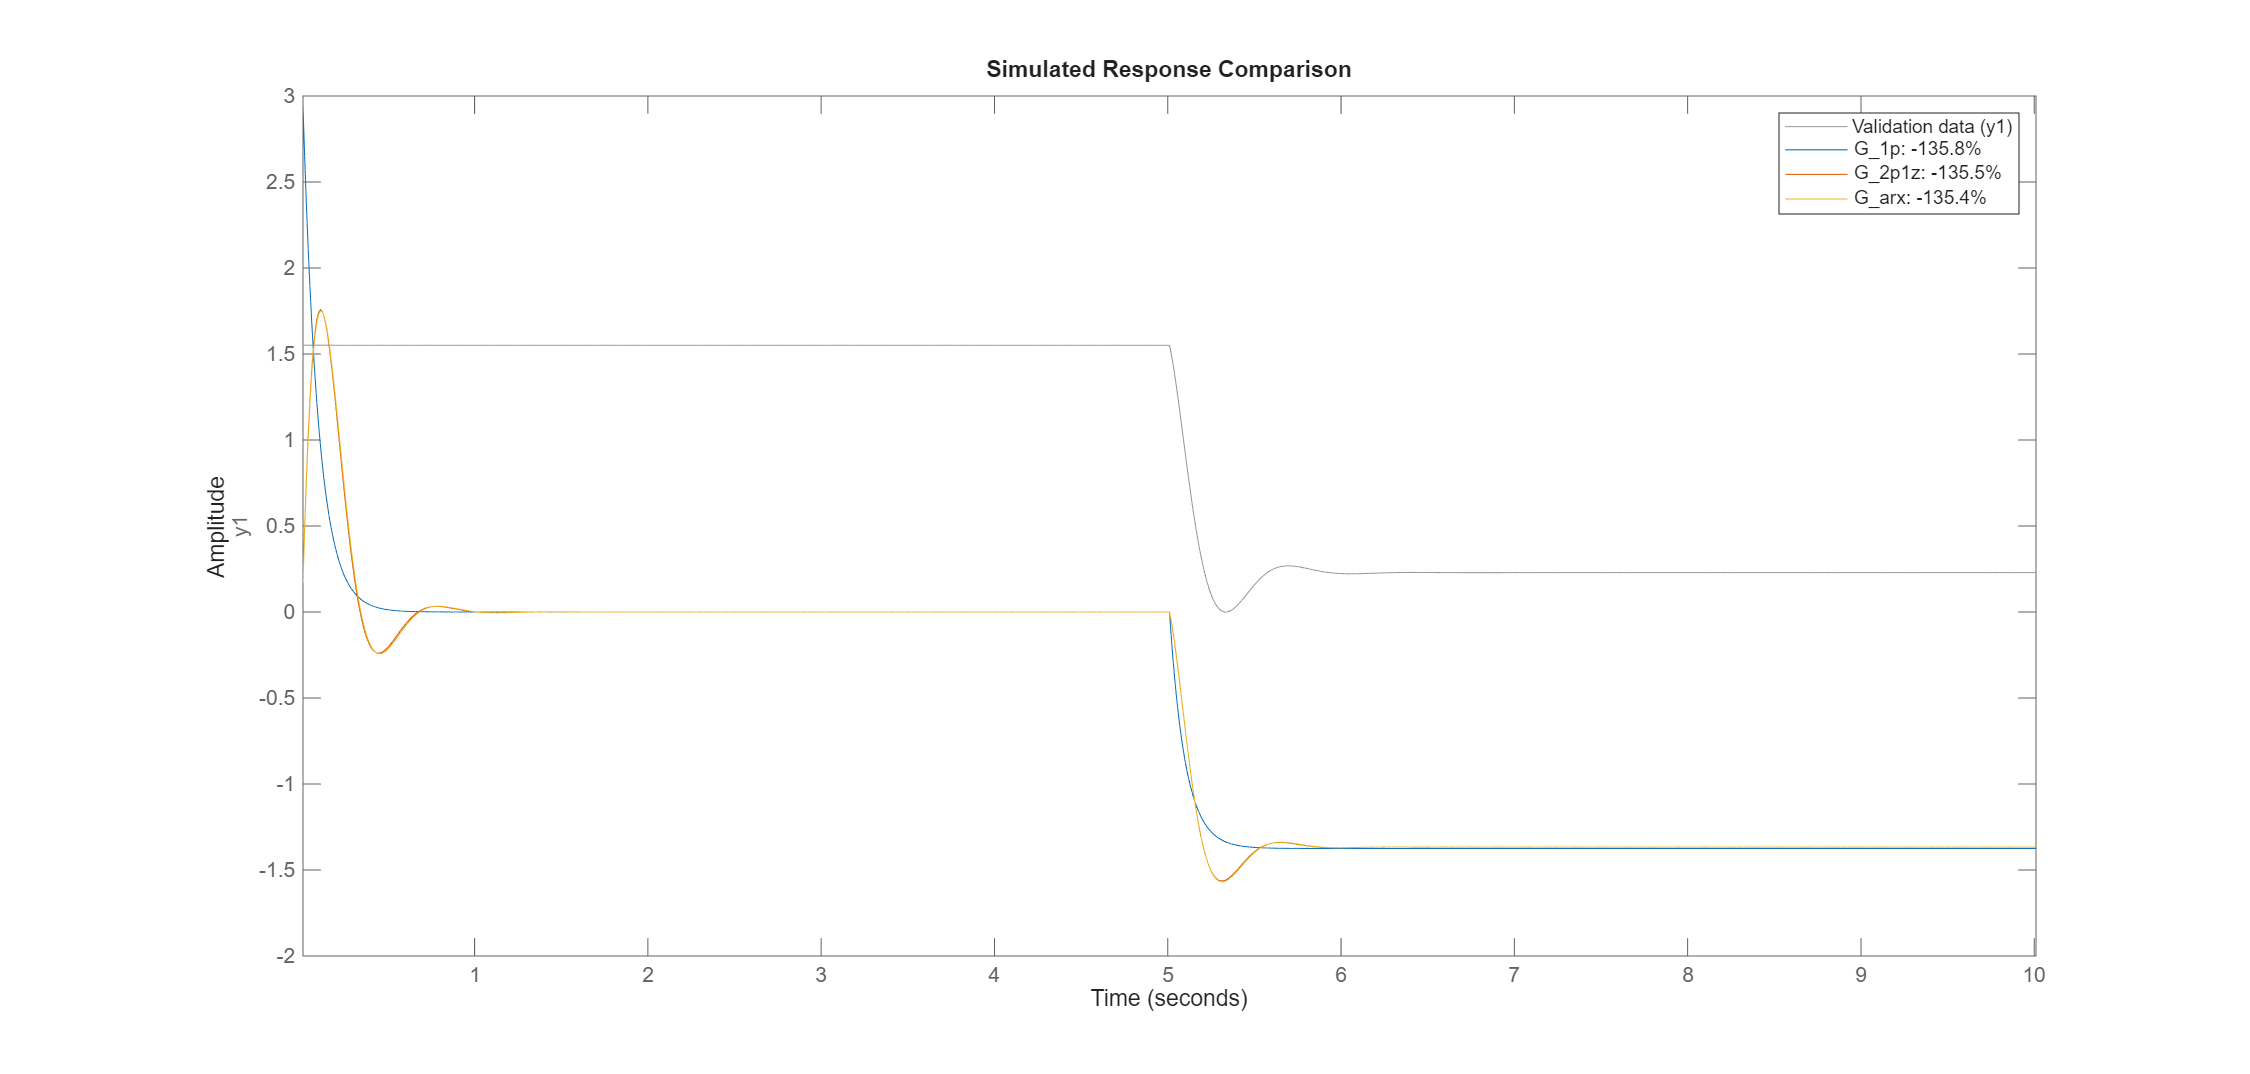
\includegraphics[width=0.8\textwidth]{../figures/1000 to 1050.png}
    \caption{Validation response for cooling water flow step from 1000 to 1050 lbmol/h.}
    \label{fig:step_response_3}
\end{figure}

It can be seen that in both cases, the system behaves as expected. Particularly the trayectory is well predicted by the second order and ARX models. The first order model is not able to predict the overshoot, and therefore, it is not a good model for the trayectory. 

All of the models have a slight deviation with respect with the estimated gain of the system. This is due to the fact that the system is nonlinear, and therefore, the gain changes with respect to the operating point.